\section{Model}
A dynamical model of the system is derived, first by Newton's method and then by the energy method. The model is based on the conventions presented in the mechanical diagram in \autoref{fig:mechanicalDrawing} while excessive coordinates are defined in \autoref{fig:excessiveCoordinates}. The cart is constrained to the horizontal rail s.t. $y_c = 0$, that is, the cart only ever moves along the $x$-axis.

%\begin{figure}[H]
%  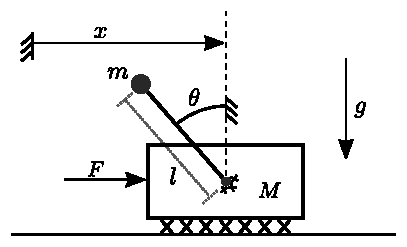
\includegraphics[width=.5\textwidth]{figures/mechanicalDrawing}
%  \caption{The cart pendulum system with generalized coordinates, $x$ and $\theta$, where $x$ is the center position of the cart, $\theta$ is the angle of the pendulum, $m$ is the point mass of the pendulum, $M$ is the mass of the cart, g is the gravitational acceleration and f is the force of actuation.}
%  \label{fig:mechanicalDrawing}
%\end{figure}

\begin{figure}[H]
  \hspace{-10pt}
  \captionbox
  {
    The cart pendulum system with excessive coordinates, where $(x_c, y_c)$ is the position of pendulum pivot point on the cart and $(x_p, y_p)$ is the position of the pendulum point mass.
    \label{fig:excessiveCoordinates}
  }
  {
    \hspace{-1cm}
    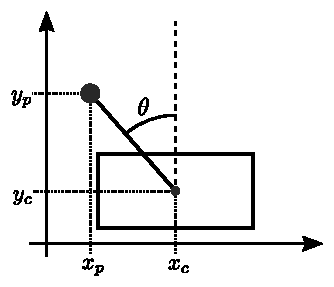
\includegraphics[width=.4\textwidth]{figures/excessiveCoordinates}\vspace{-11pt}
  }
  \hspace{20pt}
  \captionbox 
  {
    Mechanical drawing of the cart pendulum system with $x$ and $\theta$ as generalized coordinates, where $x$ is the center position of the cart, $\theta$ is the angle of the pendulum, $m$ is the point mass of the pendulum, $M$ is the mass of the cart, g is the gravitational acceleration and $F$ is the force of actuation.
    \label{fig:mechanicalDrawing}
  }
  {
    \hspace{-1cm}
    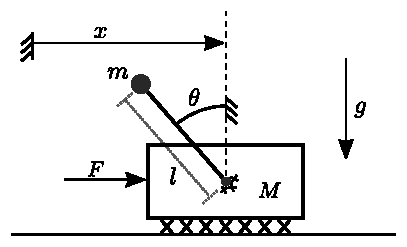
\includegraphics[width=.5\textwidth]{figures/mechanicalDrawing}\vspace{6pt}
  }  
\end{figure}


It is assumed that the pendulum rod is rigid and massless. This is deemed sensible, as the pendulum mass is much heavier than the hollow aluminum rod. The pendulum mass is modeled as a point mass placed at its geometrical center. This is why the length, $l$, is measured from the pivot point to the center of the pendulum mass.\\
The mass of the cart includes the weight of the belt and the wires hanging from the cart to the controller and supply. The influence of the wires will vary depending on the position of the cart, but this is treated as an unmodeled disturbance.\\
The frictions are assumed to consist solely of Coulomb and viscous friction. This is a fairly simplified friction model and while it might be advantageous to include further friction dynamics, such as stiction and Stribeck friction, it is considered to be out of scope in this project. Both viscous and Coulomb friction on the cart are assumed purely translational, and will therefore also include friction and inertia added by the motor and pulleys.

\fxnote{review if all assumptions are included}

\subsection{Newton's Method}

Excessive coordinates - freebody diagrams in \autoref{fig:freeBodyCart} and \ref{fig:freeBodyPendulum}

\begin{figure}[H]
  \hspace{-10pt}
  \captionbox
  {
    freeBodyCart
    \label{fig:freeBodyCart}
  }
  {
    \hspace{-1cm}
    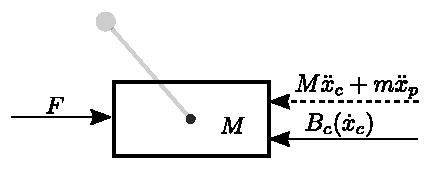
\includegraphics[width=.4\textwidth]{figures/freeBodyCart}
  }
  \hspace{20pt}
  \captionbox 
  {
    freeBodyPendulum
    \label{fig:freeBodyPendulum}
  }
  {
    \hspace{-1cm}
    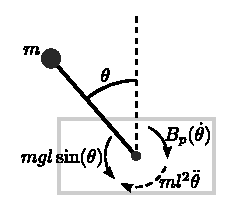
\includegraphics[width=.28\textwidth]{figures/freeBodyPendulum}
  }  
\end{figure}
%
Newton's second law for the cart along x. Freebody diagram in \autoref{fig:freeBodyCart}
\begin{flalign}
  M\ddot{x}_c + m\ddot{x}_p &= F - B_c(\dot{x}_c) &&
  \label{eq:newtonAlongX}
\end{flalign}
%
Applying Newton's second law for rotational motion. Freebody diagram in \autoref{fig:freeBodyPendulum}
\begin{flalign}
  ml^2 \ddot{\theta} &= mgl \sin \theta - B_p(\dot{\theta}) &&
  \label{eq:newtonRotation}
\end{flalign}
%
Relation of D'alumbert forces for the pendulum decomposed as tangential forces,
\begin{flalign}
  - m\ddot{x}_p \cos \theta - m\ddot{y}_p \sin \theta &= ml \ddot{\theta} &&
  \label{eq:dalumbert}
\end{flalign}
%
To combine \autoref{eq:dalumbert} and \ref{eq:newtonRotation}, \autoref{eq:dalumbert} is written as torques,
\begin{flalign}
  - ml\ddot{x}_p \cos \theta - ml\ddot{y}_p \sin \theta &= ml^2 \ddot{\theta} &&
  \label{eq:dalumbertTorques}
\end{flalign}
%
\autoref{eq:dalumbert} and \ref{eq:newtonRotation} are combined,
\begin{flalign}
  - ml\ddot{x}_p \cos \theta - ml\ddot{y}_p \sin \theta &=  mgl \sin \theta - B_p(\dot{\theta}) &&
  \label{eq:dalumbertTorquesANDnewtonRotation}
\end{flalign}
%
The system dynamics is then represented using excessive coordinates by the following set of equations:
\begin{flalign}
    \begin{cases}
      M\ddot{x}_c + m\ddot{x}_p &= F - B_c(\dot{x}_c) \\
    - ml\ddot{x}_p \cos \theta - ml\ddot{y}_p \sin \theta &=  mgl \sin \theta - B_p(\dot{\theta})
  \end{cases} &&
  \label{eq:excessiveCoordinates}
\end{flalign}
%
Writing the excessive coordinates, \autoref{fig:excessiveCoordinates}, in therms of the generalized coordinates, \autoref{fig:mechanicalDrawing},
\begin{flalign}
  \begin{cases}
    x_c &=  x  \\
    y_c &=  0  
  \end{cases}
    \hspace{20pt}
  \begin{cases}
    x_p =  x - l\sin \theta \\
    y_p =  l\cos \theta
  \end{cases}  &&
  \label{eq:coordinateTransformation}
\end{flalign}
%
Finding the derivatives for the transformation,
\begin{flalign}
  \begin{cases}
    \dot{x}_p &= \dot{x} - l\cos \theta \dot{\theta} \\
    \dot{y}_p &= -l\sin \theta \dot{\theta}
  \end{cases}
    \hspace{20pt}
  \begin{cases}
    \ddot{x}_p = \ddot{x} + l \sin \theta \dot{\theta}^2 - l\cos \theta \ddot{\theta} \\
    \ddot{y}_p = -l\cos \theta \dot{\theta}^2  -l\sin \theta \ddot{\theta}
  \end{cases}  &&
  \label{eq:transformationDerivatives}
\end{flalign}
%
Rewriting \autoref{eq:excessiveCoordinates} in generalized coordinates using the cooredinate transformation from \autoref{eq:coordinateTransformation} and \ref{eq:transformationDerivatives} yields,
\begin{flalign}
  \begin{cases}
    M\ddot{x} + m( \ddot{x} + l\sin \theta \dot{\theta}^2 - l \cos \theta \ddot{\theta} ) = F - B_c(\dot{x}) \\
    - ml( \ddot{x} + l \sin \theta \dot{\theta}^2 -l\cos \theta \ddot{\theta} ) \cos \theta - ml ( -l \cos \theta \dot{\theta}^2 -l\sin \theta \ddot{\theta} ) \sin \theta =  mgl \sin \theta - B_p(\dot{\theta})
  \end{cases} \nonumber
\end{flalign}
\vspace{-17pt}
\begin{flalign}
  \begin{cases}
  ( M + m ) \ddot{x} + ml\sin \theta \dot{\theta}^2 - ml\cos \theta \ddot{\theta} &= F - B_c(\dot{x}) \\
  - ml\cos \theta \ddot{x} + ml^2 \ddot{\theta} - mgl \sin \theta &= - B_p(\dot{\theta})  \ \ \ \ ,
\end{cases} &&
\label{eq:generalizedCoordinates}
\end{flalign}
%
which is the final dynamic equations for the cart pendulum system.

\subsection{Energy Method}

\fxnote{include friction model}
The energy method is applied to find the dynamic equations using generalized coordinates, $x$ and $\theta$, as defined in \autoref{fig:freeBody}. The kinetic energy $T$ is given by,
%
\begin{flalign}
  T &= \frac{1}{2} M \dot{x}^2 + \frac{1}{2} m (\dot{x} + l \dot{\theta} \cos \theta )^2 + \frac{1}{2} m (-l \dot{\theta} \sin \theta )^2  & \nonumber \\ % \unit{N \cdot m}\\
  T &= \frac{1}{2} (M+m) \dot{x}^2 + m \dot{x} l \dot{\theta} \cos \theta + \frac{1}{2} m l^2 \dot{\theta}^2 \ \ \ . & \unit{N \cdot m}
  \label{eq:kineticEnergy}
\end{flalign}
%
%\begin{where}
%  \va{ T                 }{is the kinetic energy}                      {N \cdot m}
%  \va{ M                 }{is the mass of the cart}                    {kg}
%  \va{ \dot{x}           }{is the velocity of the cart}                {m \cdot s^{-1}}
%  \va{ m                 }{is the mass of the pendulum}                {kg}
%  \va{ l                 }{is the length of the pendulum}              {m}
%  \va{ \theta            }{is the angle of the pendulum}               {rad}
%  \va{ \dot{\theta}      }{is the angular velocity of the}             {rad \cdot s^{-1}}
%\end{where}

The potential energy is given by,
%
\begin{flalign}
  V &= M g l \cos \theta \ \ \ . & \unit{N \cdot m}
  \label{eq:potentialEnergy}
\end{flalign}
%
\begin{where}
  \va{ V                 }{is the potential energy}                    {N \cdot m}
  \va{ g                 }{is the gravitational acceleration}          {m \cdot s^{-2}}
\end{where}

By \autoref{eq:kineticEnergy} and \autoref{eq:potentialEnergy} the Lagrangian becomes,
%
\begin{flalign}
  \cal{L} &= T - V & \nonumber \\ 
  \cal{L} &= \frac{1}{2} (M+m) \dot{x}^2 + m \dot{x} l \dot{\theta} \cos \theta + \frac{1}{2} m l^2 \dot{\theta}^2 - M g l \cos \theta \ \ \ . & \unit{N \cdot m}
  \label{eq:lagrangian}
\end{flalign}
%
\begin{where}
  \va{ \cal{L}           }{is the Lagrangian}                          {N \cdot m}
\end{where}

From the energy method we find the dynamic equations corresponding to each of the generalized coordinates, $\theta$ and $x$, by,
%
\begin{flalign}
  \frac{d}{dt} \left( \frac{\partial \cal{L}}{\partial \dot{\theta}} \right) - \frac{\partial \cal{L}}{\partial \theta} &=  0  & \\ %\unit{N \cdot m}  \\
  \frac{d}{dt} \left( \frac{\partial \cal{L}}{\partial \dot{x}} \right) - \frac{\partial \cal{L}}{\partial x} &=  f  \ \ \ . & %\unit{N \cdot m}
  \label{eq:energyMethod}
\end{flalign}
%
\begin{where}
  \va{ f          }{is the actuation force, see \autoref{fig:system}}             {N \cdot m}
\end{where}

Inserting the Lagrangian and reducing the expressions finally yields the dynamic equations,
%
\begin{flalign}
  m l \cos \theta \ddot{x} + m l^2 \ddot{\theta} - m l g \sin \theta &=  0  & %\unit{N \cdot m}  \\
  \label{eq:dynamicEquation1} \\
  (M+m) \ddot{x} + m l \cos \theta \ddot{\theta} - m l \sin \theta \dot{\theta}^2 &= f  \ \ \ . & %\unit{N \cdot m}
  \label{eq:dynamicEquation2}
\end{flalign}


\subsection{Simulation and Verification}

A block diagram is derived in \autoref{fig:blockDiagram} from \autoref{eq:dynamicEquation1} and \autoref{eq:dynamicEquation2}.

\begin{figure}[H]
  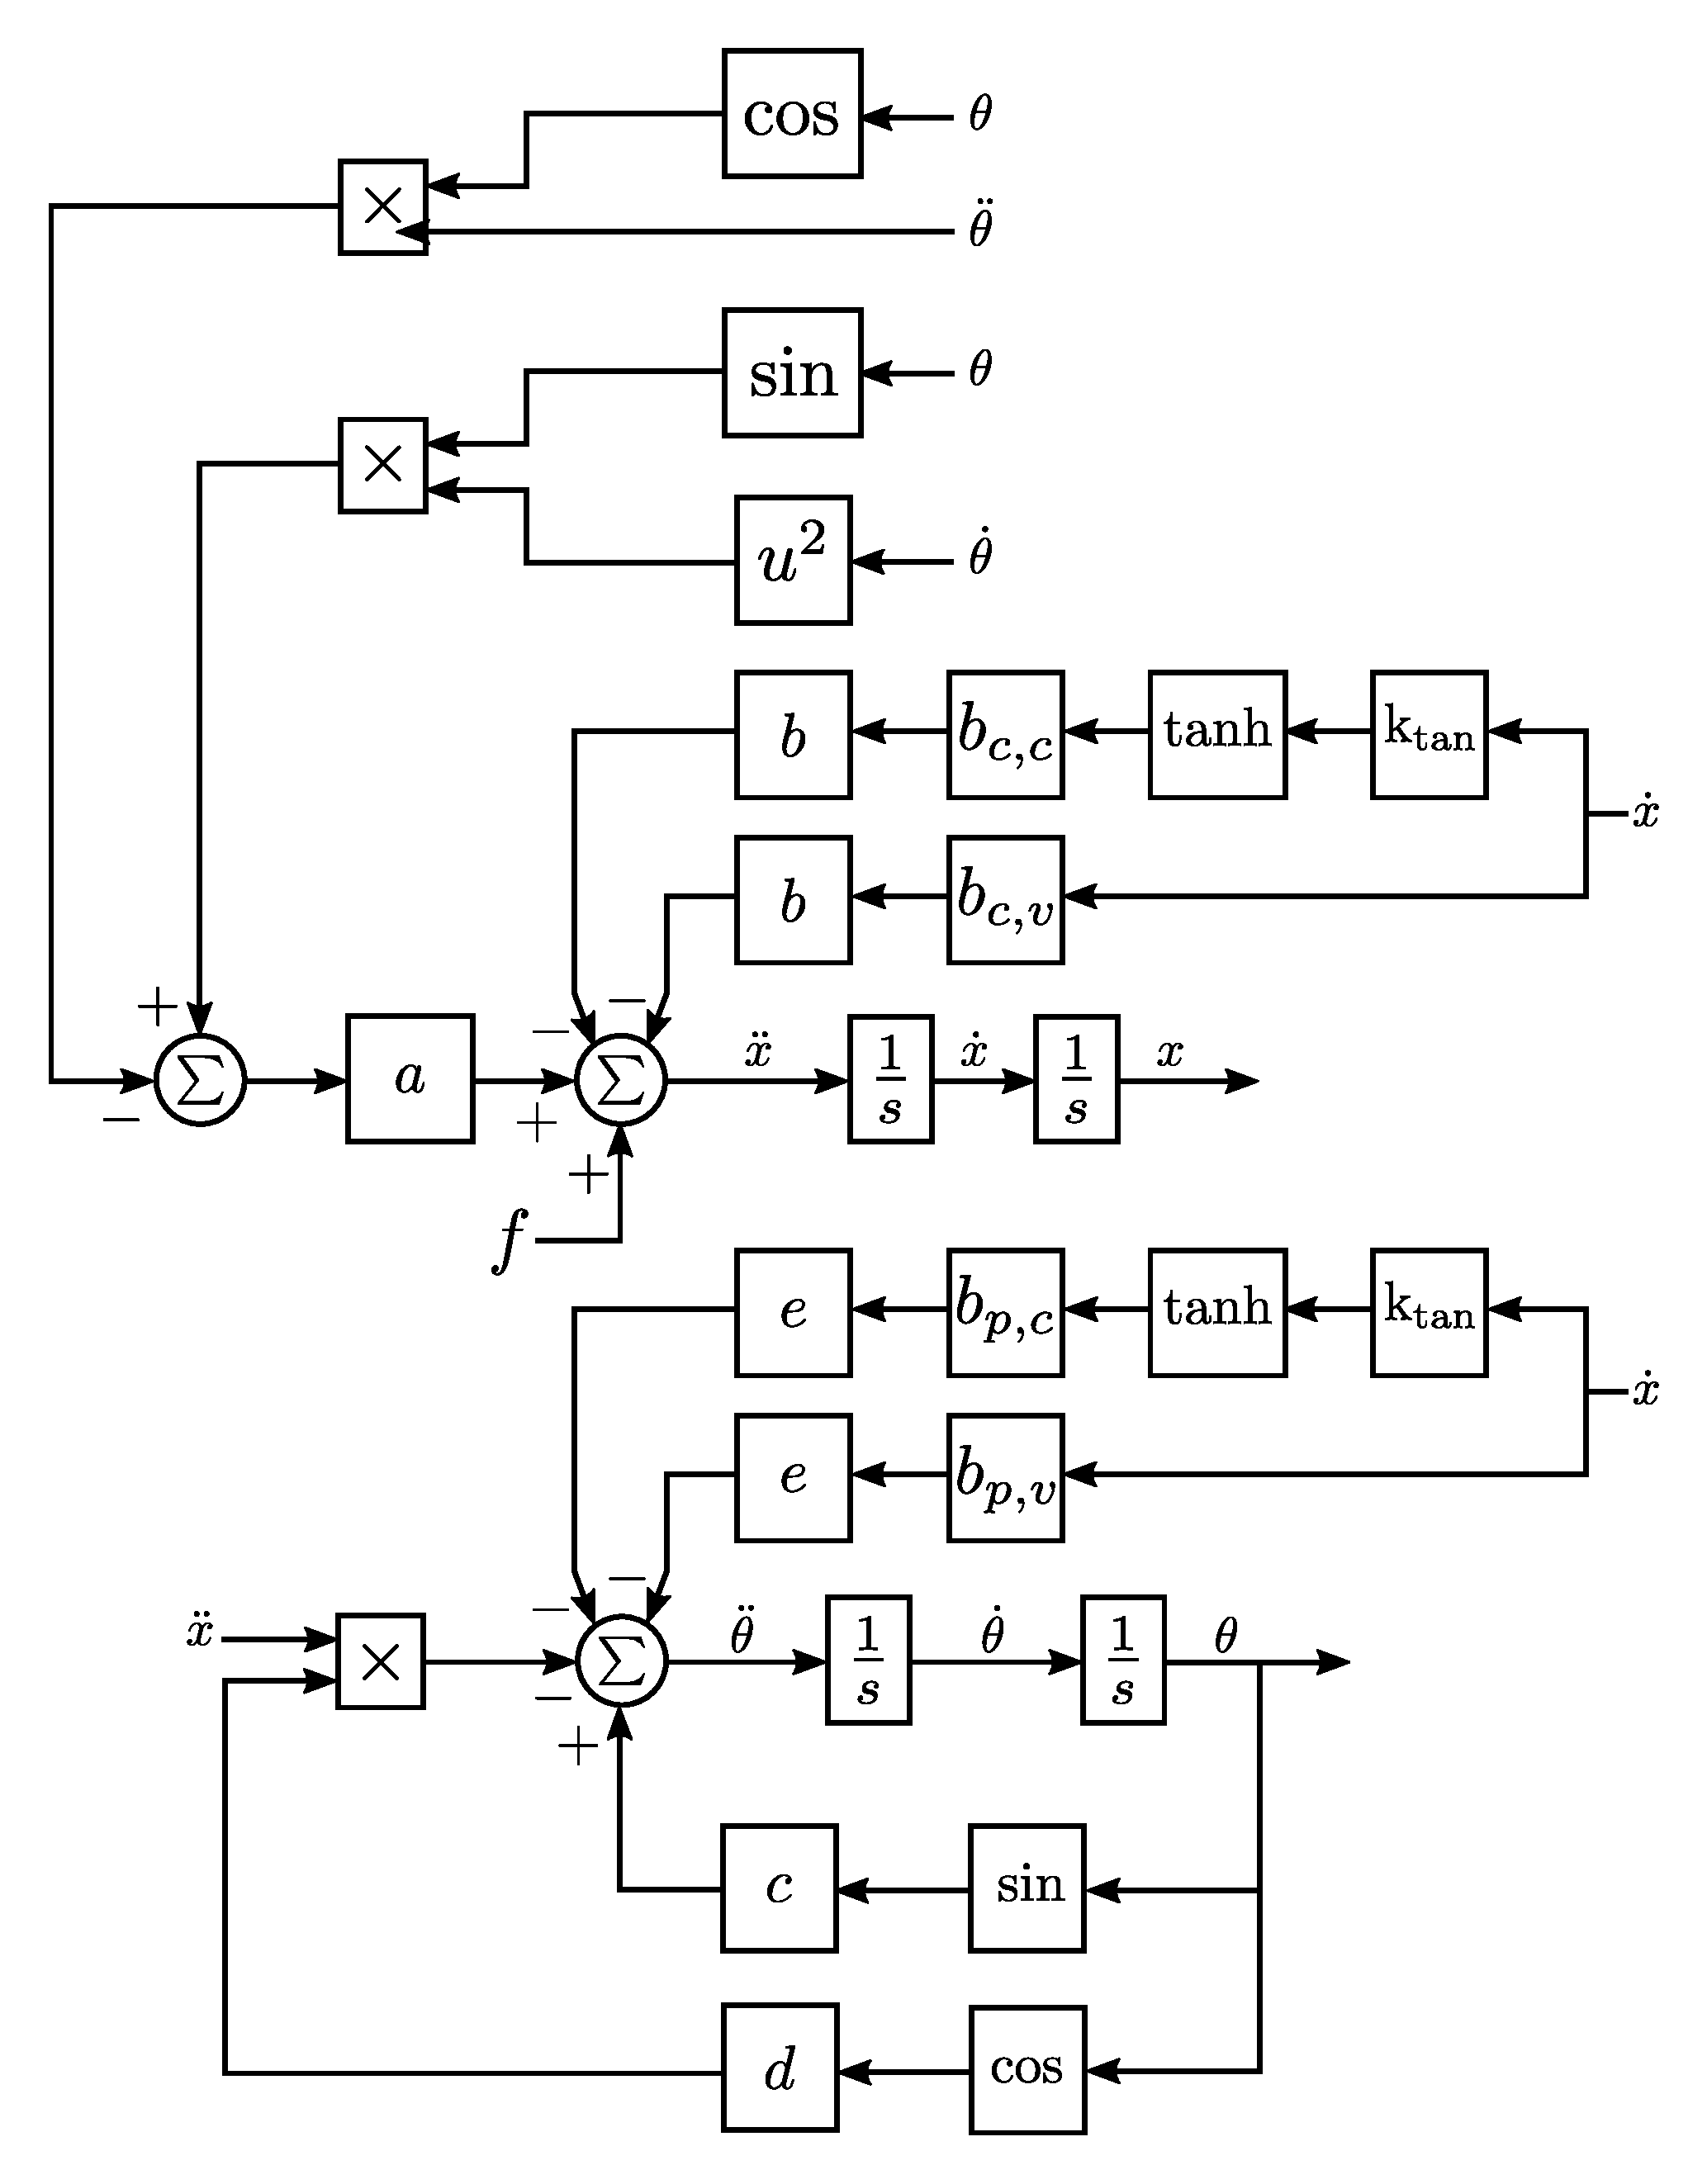
\includegraphics[width=.7\textwidth]{figures/blockDiagramWithFriction}
  \caption{A block diagram derived from the dynamic equations, later used for simulation. Five signal connections, from $\dot{\theta}$, $\ddot{\theta}$, $\ddot{x}$ and two from $\theta$, are drawn without explicit connection to keep the figure clear.}
  \label{fig:blockDiagram}
\end{figure}

This is implemented in Matlab Simulink to simulate the system. A graphical layer, including the obstacles, is added to the simulation to show the system in action.